\chapter{The communication model}

Shannon developed a mathematical model of the communication among parties. In particular, we will not consider the simplest one, in which the communication is one-way between two entities. In this model, one entity is the \emph{source} that sends information to the second entity, called the \emph{receiver}, through a \emph{noisy channel}.

\begin{figure}[h!]
	\centering
	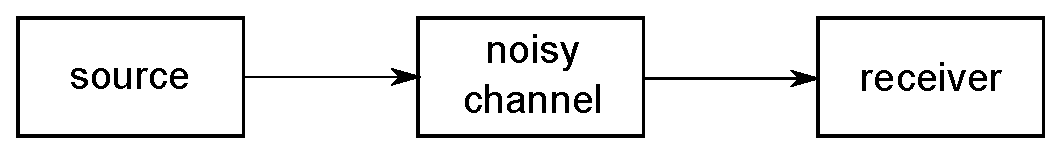
\includegraphics[width=0.6\linewidth]{pictures/comm-channel.eps}
	\caption{Graphic model of a simple communication.}
\end{figure}

Source and receiver are usually separated in space and communicate (approximately) at the same time. Indeed, the roles of space and time can be swapped (i.e. a communication that evolves over time at the same place, like data storage and retrieval).

The noisy channel is both the veicle and the obstacle. One cannot transmit a signal without it being modified to some extent; moreover the communication must be quick because time is expensive. The alterations to the message are errors and therefore must be corrected. In order to do this we need to remove ``bad'' redundancy and add ``good'' redundancy. So we have a tradeoff between data integrity and fast communication.

\begin{figure}[h!]
	\centering
	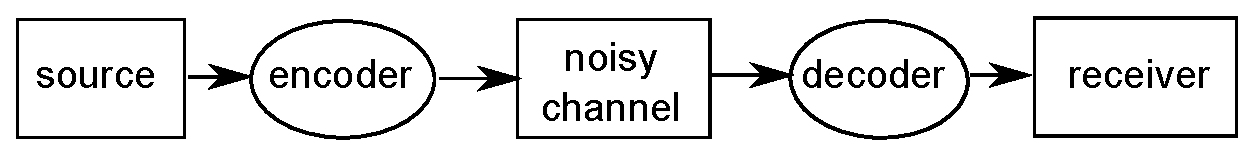
\includegraphics[width=0.9\linewidth]{pictures/comm-channel1.eps}
	\caption{The role of encoder and decoder.}
\end{figure}

The balance is found by the \emph{encoder}. This entity takes the message from the source, modify it in some way, and transmit the result over the channel. A \emph{decoder} is the entity that apply some transformation to the incoming flow of information before handling it to the receiver. The decoder can't perform the inverse of the encoder's function, because the channel applies noise to the information. We will concentrate on the noisy channel, without considering encoder and decoder's interfaces to source and receiver.

%NOTE: here he said something on asimptotic equipartition

\section{Discrete Memoryless Channel (DMC)}

For now, the channel is a black box. Let $\xset$ be the input alphabet and $\yset$ be the output alphabet for the strings that respectively enter and exit the channel. Select an input symbol $x \in \xset$; a random symbol $y \in \yset$ comes out of the channel.

We can think that there is a ``devil'' inside the black box (yes, you've read correctly, lol). The devil has dices that have $|\yset|$ faces. Whenever an input signal enters the channel, the devil launches a dice and outputs the symbol on the facet that comes up. The devil can't launch any dice; instead, there is a mapping between dices and input symbols (you can think of $x$ as the name of the dice that the devil has to use). So we can influence the devil in using some specific dice (out of the $|\xset|$ dices), but the outcome is still stochastic. The probability distribution of each dice is arbitrary. Note that the channel is usable if e have different dices; otherwise, the output is completely uncontrollable.


Let $W(y|x)$ be the probability that the dice named $x$ will fall onto its facet $y$, with the following conditions: 
\begin{itemize}
	\item 
	$W(y|x) \geq 0$,
	\item $\forall x \sum_{y \in \yset} w(y|x) = 1$.
\end{itemize}

We can think of $W$ as a matrix whose columns are indexed by $y$ and rows are indexed by $x$.

To communicate iteratively pick $x_1,x_2, \ldots, x_n \in \xset^n$ and launch a sequence of dices. There is a probability distribution for $y_1, y_2, \ldots, y_n \in Y^n$. Consider the function
\[
W^n(\str{x}, \str{y}): \xset^n \rightarrow \yset^n
\]
defined as
\[
W^n(\str{x}, \str{y}) = \prod_{i = 1}^n W(y_i | x_i)
\]

We assume that every symbol is independently modified (lack of memory of the channel). We can now define the DMC (over time instants) as
\[
\emph{DMC} = \{W^n\}_{n = 1}^\infty
\]

\section{Shannon's Noisy Channel Theorem}

The encoder takes the messages of the source and maps it to an arbitrary subset $C \subseteq \xset^n$. So we have $|C|$ many messages that flow in the channel; they can be non-binary strings, but to have an approximation of their length we can assume they are binary. Then, the length of these messages is $\log_2|C|$. We define the speed of the channel as $$\dfrac{1}{n}\log_2|C|,$$ where $n$ is the length of transmission in some unit of time. We can call this \emph{rate} of the code.

Now we are interested in the quality of transmission, that is how well data transmitted can be recovered. The decoder is a function $\varphi: \yset^n \rightarrow C$. An error event happens when $\str{x} \in \xset^n$ is transmitted and $\varphi(\str{y}) \not= \str{x}$. Define $$W^n(T|\str{x}) = \sum_{\str{y} \in T}W^n(\str{y}|\str{x}),$$

where $T \subseteq \yset$. The error probability of a string $\str{x} \in \xset^n$ is $$1 - W^n(\varphi^{-1}(\str{x})|\str{x}) = W^n(\overline{\varphi^{-1}(\str{x})}|\str{x})$$ where $$\varphi^{-1}(\str{x}) = \{\str{y}\ |\ \varphi(\str{y}) = \str{x} \}$$

Define the (maximum) error probability of the code $(C_n, \varphi_n)$ ($W^n$ is fixed) as 
\[
e_m(W^n, C_n, \varphi_n) = \max_{\str{x} \in C} W^n(\overline{\varphi^{-1}(\str{x})}, \str{x}).
\]

\begin{prop}
	$R \geq 0$ is an \emph{achievable rate} of transmission over the DMC $\{W\}$ if exists $\{(C_n, \varphi_n)\}_{n=1}^\infty$ such that:
	\begin{itemize}
		\item $\lim_{n \rightarrow \infty} \dfrac{1}{n}\log_2(|C_n|) \geq R$, and
		\item $\lim_{n \rightarrow \infty} e_m(W, C_n, \varphi_n) = 0$.
	\end{itemize}
\end{prop}

What is the highest achievable rate? $$C \subseteq \xset^n \Rightarrow \dfrac{1}{n}\log_2|C| \leq \log_2|\xset^n|$$
So the maximum achievable rate is $\log_2|\xset^n|$. Also, if $R_t \rightarrow R$ and $R_t$ is a series of values representing achievable rates, then $R$ is an achievable rate too (simple analysis, will not be demonstrated).

Shannon wondered about the highest achievable rate $C(W)$ of a given DMC $\{W\}$. He called this number \emph{capacity of the channel}. The answer came out of his intuition but it has been proved true by his students and coworkers.

Let $x \in\xset$ be a symbol chosen following a probability distribution $P|\xset$. The input symbol will be sent through the channel $W$ and the output is conditioned by $W$. Let $Y$ be the random variable (RV), $Y \in \yset$, be the output of $W$ with respect to input $X$. Then, we have a joint distribution $P, W | \xset \times \yset$. The probability that a specific input $x$ corresponds to a received symbol $y$ is
\[Pr\{X=x, Y=y\} = P(x)W(y|x).\]

Define $I(X \wedge Y)$ to be the number of bits that one can transmit over a channel in a unit of time. Intuitively, it is what $y$ retains of input $x$ (mutual information). We can maximize $I$ by controlling the probability distribution $P|\xset$ (pardon the abuse of notation): $$\max_{P|\xset}I(P, W)$$

So, what is the formula for $I$?

\[
I(X \wedge Y) = \sum_{(x, y)\in X\times Y} Pr\{X=x, Y=y\}\log_2\left(\dfrac{Pr\{X=x, Y=y\}}{Pr\{X=x\}Pr\{Y=y\}}\right) =
\]

\[
= \sum_{x \in X,  y\in Y} Pr\{X=x\}W(y|x)\log_2\left(\dfrac{Pr\{X=x\}W(y|x)}{\sum_{x\in X}Pr\{X=x\}W(y|x)}\right) = I(P, W)
\]

\begin{thm}[Shannon's Noisy Channel Theorem]\label{thm:nct}
	The highest achievable rate, given a DMC $W$, is $$C(w) = \max_{P|X}I(P, W).$$
\end{thm}

Notice that $C(W)$ is 0 if $X$ and $Y$ are independent $\Leftrightarrow$ all rows in $W$ are the same. 

\section{Binary Symmetric Channel}

A binary symmetric channel is used to transmit binary strings and the DMC has the form
\[
W = \left({\begin{array}{cc}
	1-p & p\\
	p & 1-p\\
	\end{array}}\right), \xset = \yset = \{0, 1\}
\]

It is called symmetric because $W$ is. In this context $P|\xset$ is called \emph{crossover} probability. The (hypothetical, since we proved nothing) capacity of this channel according to Theorem \ref{thm:nct} is:
\[I(X \wedge Y) = H(Y) - H(Y|X) \leq 1 -h(p)\]

This is true because:
\begin{itemize}
	\item the maximum value for $H(Y)$ is 1;
	\item the following equations hold:
	\[H(Y|X) = \sum_{x\in X}Pr\{X=x\}H(Y|X=x) = h(p),\] where 
	\[H(Y|X=x) = \sum_{y \in Y}Pr\{Y=y|X=x\}\log_2\left(\dfrac{1}{Pr\{Y=y | X=x\}} \right).\]
\end{itemize} 

Is this upper bound achievable? We must make sure that $$\exists X\ H(Y) =1$$
We can impose the uniform distribution when picking the input values, i.e. $Pr\{X = 0\} = \ifrac{1}{2}$.

We will show that $1-h(2p)$ is an achievable rate if $p < \ifrac{1}{4}$. We will do this using error correcting codes.

\begin{obs}
 $1-h(2p)$ is an achievable rate if $p < \ifrac{1}{4}$.
\end{obs}

\noindent\textbf{Ver}. Choose $\str{x} \in \{0, 1\}^n$ arbitrary, but think of $\str{0}$ (it's easier). Consider the Hamming ball $\hball{\str{0}}{n(p+\epsilon)}$; we want that $$W^n(\phi^{-1}_n(\str{0}) | \str{0}) \rightarrow 1.$$ Consider a code for which $$\forall \str{x} \in \cwset\ \phi^{-1}_n(\str{x}) \supseteq \hball{\str{x}}{n(p+\epsilon)};$$ these H-balls should be disjoint. Is it true that $$W^n(\hball{\str{0}}{n(p+\epsilon)} | \str{0}) \rightarrow 1?$$ This is what we should achieve , and prove that $np$ is a good choice. Take what you receive: $\str{x} \oplus Z^n$. We say $Z^n \cdot \str{x} \oplus Y^n$ (?).
\[
 Y^n \in \hball{\str{0}}{n(p+\epsilon)} iff Z^n \text{has at most}\ n(p+\epsilon) 1s. 
\]

\[
 \text{\#1s in }Z^n = \sum_{i=1}^n Z_i,
\]
where $Z_i \sim (1-p, p)$ is a random variable.

\[
 E(Z_i) = Pr[Z_i = 0]0 + Pr[Z_i = 1] = p
\]

$\{Z_i\}_{i=1}^n$ is an i.i.d. sequence of RVs.

\[
E(Z^n) = E(\sum_{i=1}^nZ_i) = \sum_{i=1}^nE(Z_i) = np
\]

by the law of large numbers 
\[
Pr\left[\left|\dfrac{1}{n} \sum_{i=1}^nZ_i -p \right| > \epsilon \right] \rightarrow 0
\]

the complement of this event has a probability that converges to 1. How can we guarantee that these H-balls of radius $n(p+\epsilon)$ are disjoint? This is guaranteed if $d_H(\str{x}',\str{x}'') \geq 2n(p+\epsilon)$. Thus $d_H(\cwset) \geq 2n(p+\epsilon)$. G.V. Bound says that

\[
\exists \cwset\ |\cwset | \gnsim 2^{n(1-h(\delta))},\ \delta < \ifrac{1}{2}
\]

and

\[
d_H(\cwset) \gnsim n\delta.
\]

We want $d_H(\cwset) \geq 2n(p+\epsilon)$, thus what we want is achievable iff

\[
2p + \epsilon < \dfrac{1}{2} \sim p < \dfrac{1}{4}
\]
$\hfill\Box$

Shannon stated something stronger, namely that the capacity is $1 - h(p)$. Shannon uses ``maximum likelihood''. Chooses $2^{nR}$ strings at random from $\Tau^n_p$, given $P|\xset$.

\begin{thm}[Converse part of Shannon's noisy channel coding theorem]
	If $R$ is such that $\exists \{\cwset, \cwset\}_{n=1}^\infty$ with
	$$\overline{\lim_{n \rightarrow \infty}} \dfrac{1}{n} \log|\cwset| \geq R$$
	and
	$$\lim_{n\rightarrow \infty} e_n(W^n, \cwset, \varphi) = 0$$
	then
	$$R \leq \max_{X \in \xset:P_{Y|X} = W} I(W \wedge Y).$$
\end{thm}

\noindent\textbf{Proof.} Let $M_n$ be a RV uniformly distributed over $\cwset$. Take $(\ifrac{1}{n})H(M_n)$, the average entropy.
\[
 \dfrac{1}{n})H(M_n) ) \dfrac{1}{n})\log|\cwset|
\]

to get the upper bound, we manipulate the left hand side.

\[
 \dfrac{1}{n}H(M_n) = \dfrac{1}{n}[H(M_n) - H(M_n | \varphi_n(Y^n))] + \dfrac{1}{n}H(M_n|\varphi_n(Y^n))
\]

where $Y^n$ is the RV defined by $P_{Y^n|M_n} = W^n$. In the square brackets we have a mutual information.

\[
 \dfrac{1}{n}I(M_n \wedge \varphi_n(Y^n)) + \dfrac{1}{n}H(M_n|\varphi_n(Y^n))
\]

we should be able to prove that this is not more than the upper bound. We expect the other therm to be negligible; with high probability the result of deconding the received codeword is the codeword that was sent.

\[
 I(M_n\wedge \varphi_n(Y^n)) \leq I(M_n \wedge \varphi_n(Y^n))
\]

this is from the fact that information cannot be gained by processing the RVs. We see this by looking at

\begin{equation}\label{eq:dis1}
 I(M_n\wedge \varphi_n(Y^n)) \leq I(M_n \wedge \varphi_n(Y^n)Y^n) 
\end{equation}

since

\[
 H(M_n|\varphi_n(Y^n)) \geq H(M_n|\varphi_n(Y^n)Y^n),
\]

Disequation \ref{eq:dis1} follows. The right hand side of Disequation \ref{eq:dis1} can be written as

\begin{align*}
 I(M_n \wedge \varphi_n(Y^n)Y^n) & = I(M_n \wedge Y^n) + I(M_n + \varphi_n(Y^n)|Y^n) \\ & = I(M_n \wedge Y^n).
\end{align*}

we see that

\[
 I(M_n \wedge \varphi_n(Y^n)|Y^n) \leq H(\varphi_n(Y^n)|Y^n) = 0.
\]

So we obtain the following inequality:

\[
I(M_n \wedge \varphi_n(Y^n)) \leq I(M_n \wedge Y^n) 
\]

as notation, $M_n = X_1 \leq X_n$ is a vector of random variables. Thus,

\[
 I(M_n \wedge Y^n) = I(X^n \wedge Y^n)
\]

this we want to upper bound by the conjectured value of capacity. We write
\[
 I(X^n \wedge Y^n) = H(Y^n) -H(X^n |Y^n) \leq \sum_{i=1}^n H(Y_i) - H(Y^n | X^n)
\]
for $H(Y^n | X^n)$ we use the chain rule:

\[
 H(Y^n | X^n) = \sum_{i=1}^n H(Y_i | X^nY_1\ldots Y_{i-1}).
\]

But in a discrete memoryless channel we have that
\[
 H(Y_i | X^nY_1\ldots Y_{i-1}) = H(Y_i |X_i)
\]
so
\[
 H(Y^n |X^n) = \sum_{i=1}^nH(Y_i|X_i).
\]

So what we get is that

\[
 I(X^n \wedge Y^n) = \sum_{i=1}^n I(X_i \wedge Y_i).
\]

This is true because our channel is particular.

\[
 \sum_{i=1}^n I(X_i \wedge Y_i) \leq n \max_{P_{Y|X} = W}I(X \wedge Y).
\]

which is $n$ times capacity. So:

\[
 \dfrac{1}{n}I(M_n \wedge \varphi_n(Y^n)) \leq C(W).
\]

For the second part, we have to prove that 
\[
 \dfrac{1}{n}H(M_n|\varphi_n(Y^n)) \rightarrow 0.
\]

We do so using Fano's inequality. We introduce the random variable $Z_n$ as

\begin{equation*}
Z_n = \begin{cases}
1 \text{ if }\varphi_n(Y^n) \not=M_n,\\
0  \text{ otherwise.}
\end{cases} 
\end{equation*}

We can say that
\[
 H(M_n|\varphi_n(Y^n)) \leq H(M_nZ_n | \varphi_n(Y^n))
\]
since we ``added'' something to a RV.

\begin{align*}
 H(M_nZ_n | \varphi_n(Y^n)) & = H(Z_n|\varphi_n(Y^n)) + H(M_n|\varphi_n(Y^n), Z_n)\\
 & \leq H(Z_n) + H(M_n|\varphi_n(Y^n), Z_n) \\
 & \leq 1+ H(M_n|\varphi_n(Y^n), Z_n).
\end{align*}

so, for now we have that

\[
 \dfrac{1}{n}H(M_n|\varphi_n(Y^n)) \leq \dfrac{1}{n} + \dfrac{1}{n}H(M_n|\varphi_n(Y_n), Z_n)
\]
we have to show that $$ \dfrac{1}{n}H(M_n|\varphi_n(Y_n), Z_n)$$ is small. We can break this up:

\begin{equation}\label{eq:eqbreak}
\begin{aligned}
 \dfrac{1}{n}H(M_n|\varphi_n(Y_n), Z_n) &= Pr[Z_n = 1]H(M_n|\varphi_n(Y^n), Z_n = 1) + \\
 &+ Pr[Z_n = 0]H(M_n|\varphi_n(Y^n), Z_n = 0).  
\end{aligned}
 \end{equation}
Now we have to bring in the error probability.

\begin{align*}
  & \varepsilon_n = Pr[Z_n = 1] = Pr[M_n \not=\varphi_n(Y^n)]\\
  & \leq e_n(W^n, \cwset, \varphi_n) \rightarrow 0.
\end{align*}

so $\varepsilon_n \rightarrow 0$. ``average is not more than maximum''.

\begin{align*}
 H(M_n | \varphi_n(Y^n), Z_n = 1) &= \\
 & =\sum_{y \in \yset^n} Pr[Y^n = y]H(M_n|\varphi_n(Y^n) = \varphi_n(y), Z_n = 1).
\end{align*}


$M_n \in \xset^n$. So that entropy is less than $\log|\xset^n|.$ So the first term of Equation \ref{eq:eqbreak} can be bounded by

\[
 \varepsilon_n \dfrac{1}{n}H(M_n|\varphi_n(Y^n), Z_n = 1) \leq \varepsilon_n \dfrac{1}{n} \log|\xset^n| = \varepsilon_n \log|\xset| \rightarrow 0.
\]

The second term of Equation \ref{eq:eqbreak} is equal to 0.

\[
 \dfrac{1}{n}Pr[Z_n = 0] H(M_n|\varphi_n(Y^n), Z_n = 0)
\]

to see why, note that there is no error, so $M_n = \varphi_n(Y^n).$

$\hfill\Box$

\section{Zero Error Capacity}
Zero stands for zero probability, so the probability of error is bound to be equal to 0. We translate this problem in graph theory: we will look
at product of graphs and powers of graphs. We have a DMC $\{W\},\ W:\xset \rightarrow \yset$. $W^n:\xset^n \rightarrow \yset^n$, the mathematical model of a code is the very same. A code is $(\cwset, \varphi)$ with $\cwset \subseteq \xset^n$ and $\varphi: \yset^n \rightarrow \cwset$. A code has two parameters:

\begin{itemize}
	\item $\dfrac{1}{n}|\cwset|$ is the size of the code compared to $n$. It is the number of bits transmitted over the channel per use of the channel.
	\item $e_n(W^n, \cwset, \varphi) = \max_{\str{x} \in \cwset} W^n(\overline{\varphi^{-1}(\str{x})}|\str{x})$ is the probability of error.
\end{itemize}

$(\cwset, \varphi)$ is a zero error code if $e_n(W^n, \cwset, \varphi)=0$. $R \geq 0$ is an achievable rate for error probability $0$ if $\exists (\cwset, \varphi_n)$, $\cwset \subseteq \xset^n$ with
\[
\overline{\lim_{n \rightarrow \infty}} \dfrac{1}{n}\log|\cwset| \geq R\text{ and }
\]

\[
e_n(W^n, \cwset, \varphi_n) = 0.
\]

If $W(y|x) > 0$ for all $x, y$ then this is not possible. If you have 0s in the matrix, we are only interested in the patterns of the 0s. To have 0 error, we should have that
\[
W^n(\varphi^{-1}(\str{x})|\str{x}) = 1,\ \forall\str{x} \in \cwset
\]

The decoding function must be fixed if we want $0$ error. If $W^n(\str{y}|\str{x}) \geq 0$, we must have that $\varphi^{-1}(\str{y}) = \str{x}$. Given $\str{x}$, the set $\{\str{y}| W^(\str{y}|\str{x})>0 \}$ is uniquely defined. This is the support of conditional distribution:
\begin{equation}
\supp(\str{x}) = \{\str{y}| W^n(\str{y}|\str{x})>0 \}
\end{equation}

We should have that 
\[
\supp(\str{x}) \subseteq \varphi^{-1}(\str{x}),\ \forall\str{x} \in \cwset
\]

So this,\ie how to get the 0 error probability, only depends on the set $\cwset$. Support sets have to be disjoint. $\cwset$ is a $0$ error code if
\[
\forall \{\str{x}',\str{x}'' \} \in \binom{\cwset}{2}\ \supp(\str{x}') \cap \supp(\str{x}'') = \emptyset
\]

\begin{obs}
	Let $\str{x} \in \xset^n$. Then $$\str{y} \in \supp(\str{x}) \Leftrightarrow W^n(\str{y}|\str{x}) >0,$$ but $W^n$ is a product of probabilities; thus, since
	$$W^n(\str{y}|\str{x}) = \prod_{i=1}^nW(y_i|x_i)$$
	it must be that
	$$W(y_i, x_i) > 0,\ \forall i.$$ So the support set is $$\supp(\str{x}) = \times_{i=1}^n\supp(x_i)$$
\end{obs}

This is a combinatorial condition. The support is the set of positive elements of the row of $x$. You need at least two orthogonal rows in the matrix.

\begin{obs}
	$$\supp(\str{x}') \cap \supp(\str{x}'') = \emptyset \Leftrightarrow \supp(x_i') \cap \supp(x_i'') = \emptyset,$$ for some $i$. 
\end{obs}
\noindent\textbf{Proof}. Suppose 
\begin{align*}
	&\supp(\str{x}') \cap \supp(\str{x}'') \not= \emptyset\\
	&\Leftrightarrow \exists\str{z} \in \supp(\str{x}') \cap \supp(\str{x}'')\\
	& \Leftrightarrow z_i \in \supp(x') \cap \supp(x''),\ \forall i
\end{align*}
$\hfill\Box$

Consider the graph $G = G(W)$ such that $V(G) = \xset$ and $\{x',x'' \} \in E(G)$ if $\supp(x') \cap \supp(x'') = \emptyset$. We are looking for a clique in this graph, which is the size of the best code one can have $\omega(G)$ (?) What about when we use the channel more than once? We look at $G^n = G(W^n)$, where $V(G^n) = \xset^n$ and $\{\str{x}',\str{x}''\} \in E(G^n)$ if $\exists i\ \supp(x_i') \cap \supp(x_i'') = \emptyset$. This sequence of graphs can be built using the first graph, not using always the matrix.

\noindent From $G$ to $G^n$.

\noindent Take $G$. If $\{a, b\} \in E(G)$ they are indistinguishable. Now take $G^n$. $\{\str{a}, \str{b}\} \in E(G^n)$ are indistinguishable if $\exists i \{a_i, b_i\} \in E(G)$ with $a = a_1\ldots a_n$ and $b=b_1\ldots b_n$. Every clique of maximal length is a 0 error code.

We say that 
\[
\overline{\lim_{n \rightarrow \infty}}\dfrac{1}{n}\log \omega(G^n)
\]

is the zero error capacity of $G$. This limit exists for every graph.

[MISSING 4 PAGES]



\[
 \sqrt[n]{\omega(G^n)} \geq \omega(G)
\]
\[
 C(G) = \overline{\lim_{n\rightarrow \infty}}\sqrt[n]{\omega(G^n)}
\]
That is, Shannon capacity of G.

\begin{lem}[Fevete]
Take a sequence of reals $a_n \in \Reals$, if the sequence id super additive, $\ie\ a_{m+n} \geq a_m + a_n\ \forall m, n \in \mathbb{N}$ and
\[
 \dfrac{a_n}{n} \leq M\ \forall n \in \mathbb{N}
\]

then
\[
 \exists \lim_{n \rightarrow \infty}  \dfrac{a_n}{n} 
\]

and

\[
\lim_{n \rightarrow \infty}  \dfrac{a_n}{n} = \sup_n \dfrac{a_n}{n}. 
\]
 
\end{lem}

To apply this to $\omega(G^n)$ we have to take the logarithm, since $\omega(G^n)$ is super multiplicative (and thus $\log(\omega(G^n))$ is super additive). We have that $\omega(G^n) \leq |V(G)|^n$, and thus
\[
 \dfrac{\log(\omega(G^n))}{n} \leq \log|V(G)|
\]

since 

\[
 \dfrac{a_n}{n} \leq M,\ \exists \hat{M} = \sup_n \dfrac{a_n}{n}\ \text{with}\ \hat{M} \leq M,
\]

so
\[
 \forall \epsilon\ \exists n_0\ \dfrac{a_{n_0}}{n_0} > \hat{M} - \epsilon.  
\]

Take arbitrary $n > n_0$ with $n = q_nn_0 +r_n$, with $0 \leq _n < n_0$.

\begin{align*}
 \dfrac{a_n}{n} = \dfrac{a_{q_nn_0 +r_n}}{q_nn_0 +r_n} & \geq \dfrac{q_na_{n_0} +a_{r_n}}{(q_n+1)n_0}\\
 & = \dfrac{q_n}{q_{n+1}} \dfrac{a_{n_0}}{n_0} + \dfrac{a_{r_n}}{(q_n + 1)n_0}.
\end{align*}

so the limit can be bounded from below

\[
 \underline{\lim_{n\rightarrow \infty}} \dfrac{a_n}{n} \geq \underline{\lim_{n\rightarrow \infty}}\left(\dfrac{q_n}{q_{n+1}} \dfrac{a_{n_0}}{n_0} + \dfrac{a_{r_n}}{(q_n + 1)n_0}\right) \geq \hat{M} - \epsilon
\]

(since $a_{r_n} \geq \min\{a_0, \ldots,a_{n_0 -1}\}$ the last fraction goes to 0).

$\hfill\Box$

\begin{prop}
 $$\omega(G) \leq C(G) \leq \chrom{G},$$ where $\chrom{G}$ is the chromatic number of $G$.
\end{prop}

A colouring of $G$ is a function $f: V(G) \rightarrow C$ such that if $\{a, b\} \in E(G)$ then $f(a) \not= f(b)$. $\chrom{G}$ is the minimum cardinality of $C$ such that a function $f: V(G) \rightarrow C$ like that exists.

\noindent\textbf{Proof}. 
\[
 [\omega(G)]^n \leq \omega(G^n) \leq \chrom{G^n}
\]

the first part comes from super-multiplicativity of $\omega(G)$, the second from the fact that the chromatic number of a graph is greater than the largest clique. Since $\chrom{G}$ is sub-multiplicative, we have $$\chrom{G^n} \leq [\chrom{G}]^n.$$

To show that $\chrom{G}$ is sub-multiplicative, consider an optimal colouring of $G$. $$f:V(G) \rightarrow C\ \text{with}\ |C| = \chrom{G}$$ take $\str{x} \in V(G^n)$, we colour it separately, for $x_i$ in $x_1\ldots x_n$. The function $f^n(\str{x})$, the extension by concatenation, id a correct colouring. If $\{\str{x}, \str{y}\} \in E(G^n)$, it must be that $\exists i : \{x_i, y_i\} \in E(G)$, but then, since $f(x_i) \not=f(y_i)$, $f^n(\str{x}) \not= f^n(\str(y))$. Also, the number of colours used by $f^n$ id no more than $|C^n| = [\chrom{G}]^n$, so
\[
 \omega(G) \leq \sqrt[n]{\omega(G^n)} \leq \chrom{G}
\]

$\hfill\Box$

[Note: There is a simple upper bound that is better than this. You use the ``fractional'' chromatic number. You express colouring as PU (?) and drop integer constant.]

\begin{cor}
 $$\omega(G) = \chrom{G} \Rightarrow C(G) = \omega(G).$$
\end{cor}

The corollary doesn't give us much. You can make any graph like this. Schutzenberger + Berge showed some classes of graphs for which this holds. One example is graphs for which vertices are intervals, and intersecting intervals share and edge. Furthermore, $\forall G' \subseteq G$ induced $\omega(G') = \chrom(G')$, for interval graphs.

\begin{definition}
 $G$ id perfect if $$\omega(G') = \chrom{G'}\ \forall G' \subseteq G,$$ where $G'$ is an induced subgraph.
\end{definition}

What makes this definition beautiful are two conjectures, by Berge. By now they are both theorems.
\begin{itemize}
 \item \textbf{Weak}: $G$ is perfect $\Leftrightarrow \overline{G}$ is perfect.
 \item \textbf{Strong}: minimally imperfect graphs are either odd cycles or their complements.
\end{itemize}

\begin{definition}
 A graph $G$ is minimally imperfect if
 \begin{enumerate}
  \item $G$ is not perfect, \ie $\omega(G) < \chrom{G}$,
  \item $\forall G' \subseteq G$ induced subgraph, $G'$ is perfect, \ie $\omega(G') = \chrom{G'}$.
 \end{enumerate}

\end{definition}




